\chapter{Background}
\label{chp:background}
%Background (10- 20 pages).  This should form the bulk of the interim report.
%You should consider that your objective here is to produce a near final
%version of the background section, as it will appear in your final report. 
% All of this material should be re-usable, so it is worth getting it right at
% this stage of the project.  The details of what to include can be found in
% the Project Report guidelines.

\section{Graphs}

Throughout the project we will be concerned with the study of networks represented by simple, undirected graphs. We therefore need to give the following basic definitions about graphs:

\begin{mydef}
 A graph is a pair $G = (V,E)$ composed of a finite set of vertices or nodes $V$ and a set of edges $E$.
\end{mydef}

\begin{mydef}
An isomorphism $f$ from a graph $G$ to $H$ is a bijective function $f:V(G) \to V(H)$ such that $\forall x,y \in V(G)$ there is an edge of $G$ between $x$ and $y$ if and only if there is an edge of $H$ between $f(x)$ and $f(y)$.
\end{mydef}

\begin{mydef}
An automorphism of a graph $G$ is an isomorphism from $G$ to itself.
\end{mydef}

An isomorphism is a function that maps vertices and edges from a graph $G$ to a different graph $H$, while an automorphism is a function that maps a graph $G$ to itself. Now that graphs have been introduced, we need to give the following definitions that will eventually introduce the concept of an \emph{automorphism orbit}:

\begin{mydef}
Two graphs $G$ and $H$ are called isomorphic if and only if there exists an isomorphism from $G$ to $H$.
\end{mydef}

\begin{mydef}
\label{def:non_iso}
A set of graphs $S$ is called non-isomorphic if and only if there is no isomorphism between any two graphs from $S$.
\end{mydef}

\begin{mydef}
The automorphisms of a graph $G$ form a group $Aut(G)$ called the automorphism group of $G$.
\end{mydef}

\begin{mydef}
\label{def:automorphism_orbit}
For a node $x$ of a graph $G$, the automorphism orbit of $x$ is defined as $Orb(x)=\{y \in V(G) | y = f(x) \text{ for some } f \in Aut(G)\}$
\end{mydef}

The automorphism orbits of a node $x$ in graph $G$ can be intuitively understood as the set of nodes similar to $x$ that can be interchanged with it in an automorphism. This definition is needed later on for the definition of the \emph{Graphlet Degree Vector} (see section \ref{sec:gdv}).


\begin{mydef}
 A subgraph $H=(V',E')$ of a graph $G=(V,E)$ is a graph such that $V' \subseteq V$ and $E' \subseteq E$
\end{mydef}

\begin{mydef}
\label{def:induced}
 Let $G$ be a graph and $H$ be a subgraph of $G$. $H$ is said to be induced (or full) if, for any pair of vertices $x$ and $y$ of $H$, $xy$ is an edge of $H$ if and only if $xy$ is an edge of $G$.
\end{mydef}

The definitions for non-isomorphic and induced subgraphs are needed later on in order to define what a graphlet is (see section \ref{sec:graphlets}). 

\subsection{Graph terminology}
\label{graph_terminology}

We shall now explain several commonly-used graph types and the terminology used to describe them. These will be used throughout the project when interpreting results from the Pearson GCV correlation matrices. The graph types are as follows:
\begin{itemize}
 \item cycle $S_n$: a sequence of $n$ vertices that starts and ends at the same vertex.
 \item path $P_n$: a sequence of $n$ vertices.
 \item clique $K_n$: a graph of $n$ vertices where every pair of vertices is connected by an edge.
 \item claw $C_n$: a graph of $n$ vertices that has one central node and $n-1$ satellite nodes connected to it. The satellite nodes have no edges between them.
 \item bipartite-graph: a graph whose vertices can be split into two sets $U$ and $V$ such that every edge connects one node from $U$ to a different node from $V$.
\end{itemize}

These structures will be used throughout the project in order to group graphlets\footnote{small induced subgraphs; they will be defined later on} that have common properties. A few basic graph structures are show in figure \ref{graph_terminology_pic}.

\begin{figure}[H]
\begin{center}
\begin{subfigure}{.2\textwidth}
	\begin{tikzpicture}[scale=1.0,auto,swap]

	  % define the round nodes
	  \foreach \pos/\name/\label in {
	    {(-2.0,1.46)/1/1a},
	    {(-3.5,0.5)/2/2a},
	    {(-2.5,0.5)/3/3a},
	    {(-2.0,-0.46)/4/4a}}
	    \node[vertex] (\label) at \pos {$\name$} ;

	  %neighbouring graph
		
	  \path[hi, line width=1.0]  (1a)  -- (3a);
	  \path[hi, line width=1.0]  (2a)  -- (3a);
	  \path[hi, line width=1.0]  (4a)  -- (3a);
    
	\end{tikzpicture}
	\caption{Claw}
	\label{fig:claw}
\end{subfigure}%
\begin{subfigure}{.2\textwidth}
	\begin{tikzpicture}[scale=1.0,auto,swap]

	  % define the round nodes
	  \foreach \pos/\name/\label in {
	    {(-2.0,1.46)/1/1a},
	    {(-3.5,0.5)/2/2a},
	    {(-2.0,-0.46)/3/3a}}
	    \node[vertex] (\label) at \pos {$\name$} ;

	  %neighbouring graph
		
	  \path[hi, line width=1.0]  (1a)  -- (2a);
	  \path[hi, line width=1.0]  (2a)  -- (3a);
	  \path[hi, line width=1.0]  (3a)  -- (1a);

	\end{tikzpicture}
	\caption{Cycle}
	\label{fig:cycle}
\end{subfigure}%
\begin{subfigure}{.2\textwidth}
	\begin{tikzpicture}[scale=1.0,auto,swap]

	  % define the round nodes
	  \foreach \pos/\name/\label in {
	    {(-3.0,1)/1/1a},
	    {(-2.0,0)/2/2a},
	    {(-1.0,-1)/3/3a}}
	    \node[vertex] (\label) at \pos {$\name$} ;

	  %neighbouring graph
		
	  \path[hi, line width=1.0]  (1a)  -- (2a);
	  \path[hi, line width=1.0]  (2a)  -- (3a);

	\end{tikzpicture}
	\caption{Path}
	\label{fig:path}
\end{subfigure}%
\begin{subfigure}{.2\textwidth}
	\begin{tikzpicture}[scale=1.0,auto,swap]

	  % define the round nodes
	  \foreach \pos/\name/\label in {
	    {(-2.0,1.46)/1/1a},
	    {(-3.5,0.5)/2/2a},
	    {(-2.5,0.5)/3/3a},
	    {(-2.0,-0.46)/4/4a}}
	    \node[vertex] (\label) at \pos {$\name$} ;

	  %neighbouring graph
		
	  \path[hi, line width=1.0]  (1a)  -- (2a);
	  \path[hi, line width=1.0]  (1a)  -- (3a);
	  \path[hi, line width=1.0]  (1a)  -- (4a);
	  \path[hi, line width=1.0]  (2a)  -- (3a);
	  \path[hi, line width=1.0]  (2a)  -- (4a);
	  \path[hi, line width=1.0]  (4a)  -- (3a);

	\end{tikzpicture}
	\caption{Clique}
	\label{fig:clique}
\end{subfigure}%
\end{center}
\caption[Graph types: claw, triangle, cycle and clique]{From left to right: A claw of 4 nodes ($C_4$), cycle of 3 nodes ($S_3$) (or triangle), a path of 3 nodes ($P_3$), a clique of 4 nodes ($K_4$).}
\label{graph_terminology_pic}
\end{figure}


\section{Global Network properties}

Global network properties give an overall picture of the network, but are unable to 
capture low-level patterns in the structure of the network. In the
following sections we will present a few key global properties such as the \emph{degree
distribution}, \emph{clustering coefficient} and the \emph{average path length}.

\subsection{Degree Distribution}

% \begin{figure}[h]
%   \centering
% 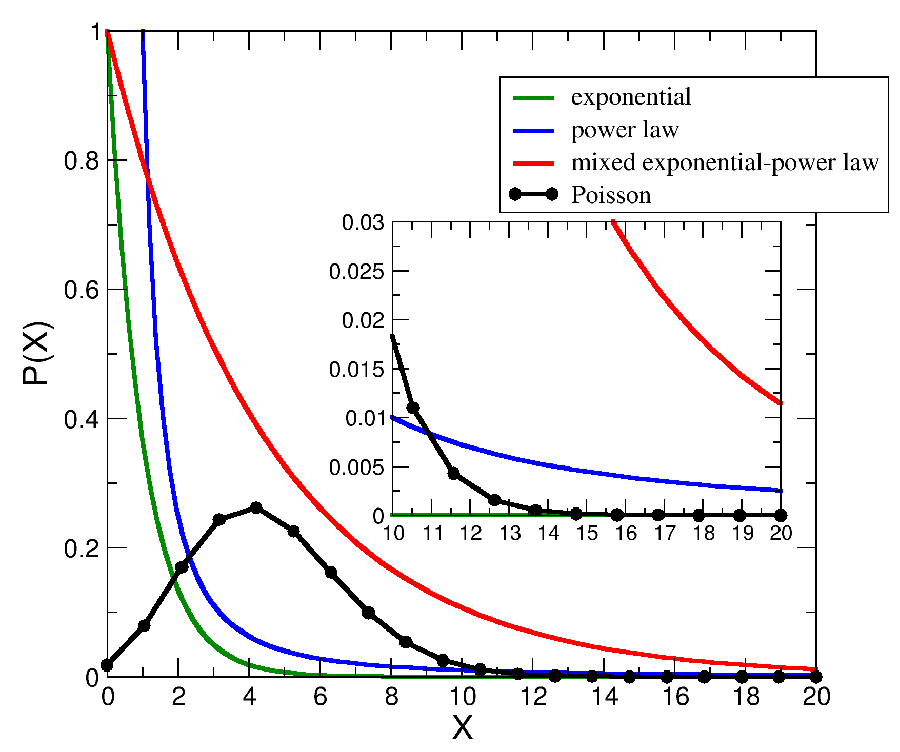
\includegraphics[scale=0.66]{images/deg_dist_all.png}
% \caption[Degree distributions: Poission, Power-law and Exponential.]{Some common classes of degree distributions:
% Poisson, Power-law and Exponential. Image source: \cite{dist2014proopnarine}}
% \label{fig:deg_dist_all}
% \end{figure}

\begin{mydef}
The degree of a node $x$ in a graph $G$ is the number of edges incident to the node, with loops counted twice. 
\end{mydef}

\begin{mydef}
The degree distribution $P(k)$ of a graph is the fraction of nodes in the network
having degree $k$. 
\end{mydef}

Several classes of degree distributions exist, with some most commonly-used ones being: 
\begin{itemize}
 \item Binomial
 \item Poison
 \item Power-law
 \item Exponential
\end{itemize}

% See figure \ref{fig:deg_dist_all} for an illustration of a Poison, Exponential and Power-law distributions. 

\begin{mydef}
A random variable $X$ follows the Bionomial distribution with parameters $n$ and $p$ if its probability mass function is given by:
$$ f(k;n,p) = {n \choose k} p^k (1-p)^{n-k}$$
\end{mydef}

\begin{mydef}
A random variable $X$ follows the Poisson distribution with parameter $\lambda > 0$ if its probability mass function is given by:
$$ f(k;\lambda) = \frac{\lambda^k e^{-\lambda}}{k!}$$
\end{mydef}

\begin{mydef}
A random variable $X$ follows the Power-law distribution with parameter $\gamma$ if its probability mass function is given by:
$$ f(k;\lambda) = k^{-\gamma}$$
\end{mydef}

A Power-law degree distribution has a high number of nodes with low degree and a very small number of nodes with high degree, also called hub nodes.

\begin{mydef}
A random variable $X$ follows the Exponential distribution with parameter $\lambda > 0$ if its probability mass function is given by:
$$ f(k;\lambda) = \lambda e^{-\lambda k}$$
\end{mydef}

Although many random graphs have a Poison degree distribution, it has been shown
that many real networks actually have a Power-law degree distribution instead. Such
networks include metabolic networks \cite{jeong2000large}, the Internet \cite{faloutsos1999power} and social networks \cite{adamic2001search}.

\subsection{Clustering Coefficient}

\begin{figure}[H]
\begin{center}
\begin{subfigure}{.3\textwidth}
  \centering
  \begin{tikzpicture}[scale=1.0,auto,swap]

    % define the round nodes
    \foreach \pos/\name/\label in {
      {(-0.0,2.0)//2a},
      {(-1.5,0.5)//3a},
      {(-1.0,-1.5)//4a},
      {(1.0,-1.5)//5a},
      {(1.5,0.5)//6a}}
      \node[vertex2] (\label) at \pos {$\name$} ;
	      
    \foreach \pos/\name/\label in {
      {(-0.0,0.0)/1/1a}}
      \node[vertex] (\label) at \pos {$\name$} ;
      
    %neighbouring graph
	  
    \path[hi, line width=1.0]  (1a)  -- (2a);
    \path[hi, line width=1.0]  (1a)  -- (3a);
    \path[hi, line width=1.0]  (1a)  -- (4a);
    \path[hi, line width=1.0]  (1a)  -- (5a);
    \path[hi, line width=1.0]  (1a)  -- (6a);

  \end{tikzpicture}
  \caption{}
  \label{fig:clust1}
\end{subfigure}%
\begin{subfigure}{.3\textwidth}
  \centering
  \begin{tikzpicture}[scale=1.0,auto,swap]

    % define the round nodes
    \foreach \pos/\name/\label in {
      {(-0.0,2.0)//2a},
      {(-1.5,0.5)//3a},
      {(-1.0,-1.5)//4a},
      {(1.0,-1.5)//5a},
      {(1.5,0.5)//6a}}
      \node[vertex2] (\label) at \pos {$\name$} ;
	      
    \foreach \pos/\name/\label in {
      {(-0.0,0.0)/1/1a}}
      \node[vertex] (\label) at \pos {$\name$} ;
      
    %neighbouring graph
	  
    \path[hi, line width=1.0]  (1a)  -- (2a);
    \path[hi, line width=1.0]  (1a)  -- (3a);
    \path[hi, line width=1.0]  (1a)  -- (4a);
    \path[hi, line width=1.0]  (1a)  -- (5a);
    \path[hi, line width=1.0]  (1a)  -- (6a);
    \path[hi, line width=1.0]  (2a)  -- (3a);
    \path[hi, line width=1.0]  (4a)  -- (5a);
    \path[hi, line width=1.0]  (4a)  -- (3a);
    \path[hi, line width=1.0]  (2a)  -- (5a);

  \end{tikzpicture}
  \caption{}
  \label{fig:clust2}
\end{subfigure}%
\begin{subfigure}{.3\textwidth}
  \centering
  \begin{tikzpicture}[scale=1.0,auto,swap]

    % define the round nodes
    \foreach \pos/\name/\label in {
      {(-0.0,2.0)//2a},
      {(-1.5,0.5)//3a},
      {(-1.0,-1.5)//4a},
      {(1.0,-1.5)//5a},
      {(1.5,0.5)//6a}}
      \node[vertex2] (\label) at \pos {$\name$} ;
	      
    \foreach \pos/\name/\label in {
      {(-0.0,0.0)/1/1a}}
      \node[vertex] (\label) at \pos {$\name$} ;
      
    %neighbouring graph
	  
    \path[hi, line width=1.0]  (1a)  -- (2a);
    \path[hi, line width=1.0]  (1a)  -- (3a);
    \path[hi, line width=1.0]  (1a)  -- (4a);
    \path[hi, line width=1.0]  (1a)  -- (5a);
    \path[hi, line width=1.0]  (1a)  -- (6a);
    \path[hi, line width=1.0]  (2a)  -- (3a);
    \path[hi, line width=1.0]  (2a)  -- (4a);
    \path[hi, line width=1.0]  (2a)  -- (5a);
    \path[hi, line width=1.0]  (2a)  -- (6a);
    \path[hi, line width=1.0]  (3a)  -- (4a);
    \path[hi, line width=1.0]  (3a)  -- (5a);
    \path[hi, line width=1.0]  (3a)  -- (6a);
    \path[hi, line width=1.0]  (4a)  -- (5a);
    \path[hi, line width=1.0]  (4a)  -- (6a);
    \path[hi, line width=1.0]  (5a)  -- (6a);

  \end{tikzpicture}
  \caption{}
  \label{fig:clust3}
\end{subfigure}%
\end{center}
\caption[Clustering coefficient example]{The clustering coefficient intuitively describes how densely connected
the neighbours of a node are. In the above three scenarios, the
clustering coefficient $C$ of node 1 increases from $C = 0$ (image \subref{fig:clust1}) to 
$C = 1$ (image \subref{fig:clust3}) as more edges are added in its neighbourhood.}
\label{fig:clustering_coeff}
\end{figure}


The clustering coefficient is another important property of a graph that is used
for data analysis and comparisons. It measures the tendency of nodes to
cluster together, which is commonly seen in social networks.

Watts and Strogatz gave the following definition to the clustering coefficient \cite{watts1998collective}:
\begin{mydef}
 Let $G$ be a graph and $n$ a node that has $k_n $ neighbours. The maximum number of edges between the neighbours of $n$ is $
\frac{k_n (k_n - 1)}{2} $. The clustering coefficient of node $n$ is then defined 
as the fraction $ C_n $ of these edges that
are present in the set of neighbours of $n$. $ C_n $ can also be viewed as the
probability of two neighbours of $n$ being connected. This is then averaged
against all the nodes in the graph and the final clustering coefficient $C$ of
graph $G$ is obtained.  
\end{mydef}

It has been shown that real networks such as metabolic networks have a high clustering coefficient \cite{ravasz2002hierarchical}. Later on we will see that some random networks such as the Erd\H{o}s-R\'{e}nyi graphs have a low clustering coefficient when the
probability $p$ of connecting two nodes is also low. This makes these models unsuitable for modeling real data.

\subsection{Average path length}

\begin{mydef}
 Let $G =(V,E)$ be a graph and $u$ and $v$ two nodes in $V$. The distance between $u$ and $v$ is defined as the smallest number of links that have to be traversed to get from $u$ to $v$.
\end{mydef}

\begin{mydef}
 Let $G =(V,E)$ be a graph. The average path length of $G$ is the average distance between any pair of two nodes from $V$. 
\end{mydef}

Real networks have been shown to exhibit a small average path length. As a result, random network models that have been developed aimed at producing networks with a small average path length. Moreover, this property has several real-life applications. For example, in a real network such as the World Wide Web, a short average path length will facilitate the exchange of information and reduce operating costs. Similarly, a power grid will suffer less losses if its average path length is minimal.  \\


\subsection{Spectral Distribution}

Spectral network theory explains the topology of a network in terms of the eigenvalues and eigenvectors of matrices associated with the network, such as the adjacency matrix or Laplacian matrix. In order to understand the spectral distribution of a network we first need to define its Laplacian matrix.

\begin{mydef}
 Let $G = (V,E)$ be an unweighted graph and let $A$ be its adjacency matrix. The diagonal degree matrix $D$ of $G$ is a matrix where the diagonal entries are equal to the node degrees, that is $D(x,x) = d_x$, where $d_x$ is the degree of node $x$. The Laplacian matrix of $G$ is defined as:
 $$ L = D - A$$
\end{mydef}

\begin{mydef}
 Let $G$ be a graph and $L$ its Laplacian matrix. The spectral distribution of $G$ is defined as the ordered vector $\lambda = (\lambda_1, \lambda_2, \dots, \lambda_n)$ of eigenvalues of $L$ , where $\lambda_1$ is the largest eigenvalue and $\lambda_n$ the smallest.
\end{mydef}


The \emph{Spectral distance} between two graphs $G$ and $H$ is then defined as the Euclidean distance of their spectral distributions. Wilson and Zhou have analysed the spectral distribution of various networks and showed that the spectral distance of two networks is the best measure for classification and clustering purposes \cite{wilson2008study}. Thorne and Strumpf have also used the spectral distribution for the analysis of the evolution of PPI networks \cite{thorne2012graph}.

\section{Local Network properties}

Local network properties capture detailed information about a local region in the network or even about one single node of interest in the network. However, local properties cannot give an overall description of the network in the way the global properties such as the degree distribution or the average path length do. In the next few sections we will
present three main types of local network properties: \emph{Node centralities}, \emph{Graphlet
Frequency Vector} and \emph{Graphlet Degree Vector}

\subsection{Node centralities}

One commonly used property for measuring the importance of a node in a
network is the centrality. Several types of centralities exist:
\begin{itemize}
 \item \emph{Degree centrality}: Measures the number of links that connect with the
node. It is simply defined as the degree of the node.
 \item \emph{Betweenness centrality}: Quantifies how many shortest paths pass through
the node
 \item \emph{Closeness centrality}: Measures how close the node is to the other nodes
in the network.
\end{itemize}

\begin{mydef}
Let $G=(V,E)$ be a graph and $v$ a node from $V$. The Degree centrality of $v$ is defined as the degree of $v$.
\end{mydef}

\begin{mydef}
Let $G=(V,E)$ be a graph and $v$ a node from $V$. The Betweenness centrality of $v$ is defined as:
$$ B(v) = \sum_{s \ne v \ne t \in V}\frac{\sigma_{st}(v)}{\sigma_{st}}$$
where $\sigma_{st}(v) $ is the number of shortest paths from $s$ to $t$ that pass
through node $v$, while $ \sigma_{st} $ is the total number of shortest paths
from $s$ to $t$.
\end{mydef}


\begin{mydef}

Let $G=(V,E)$ be a graph, $v$ a node from $V$ and $d_v$ be the sum of the distances from $v$ to
all the other nodes in the network. The Closeness centrality $C_v$ is
defined as $C_v = d_v^{-1}$. 
\end{mydef}


\subsection{Graphlets}
\label{sec:graphlets}

\begin{figure}[h]
  \centering
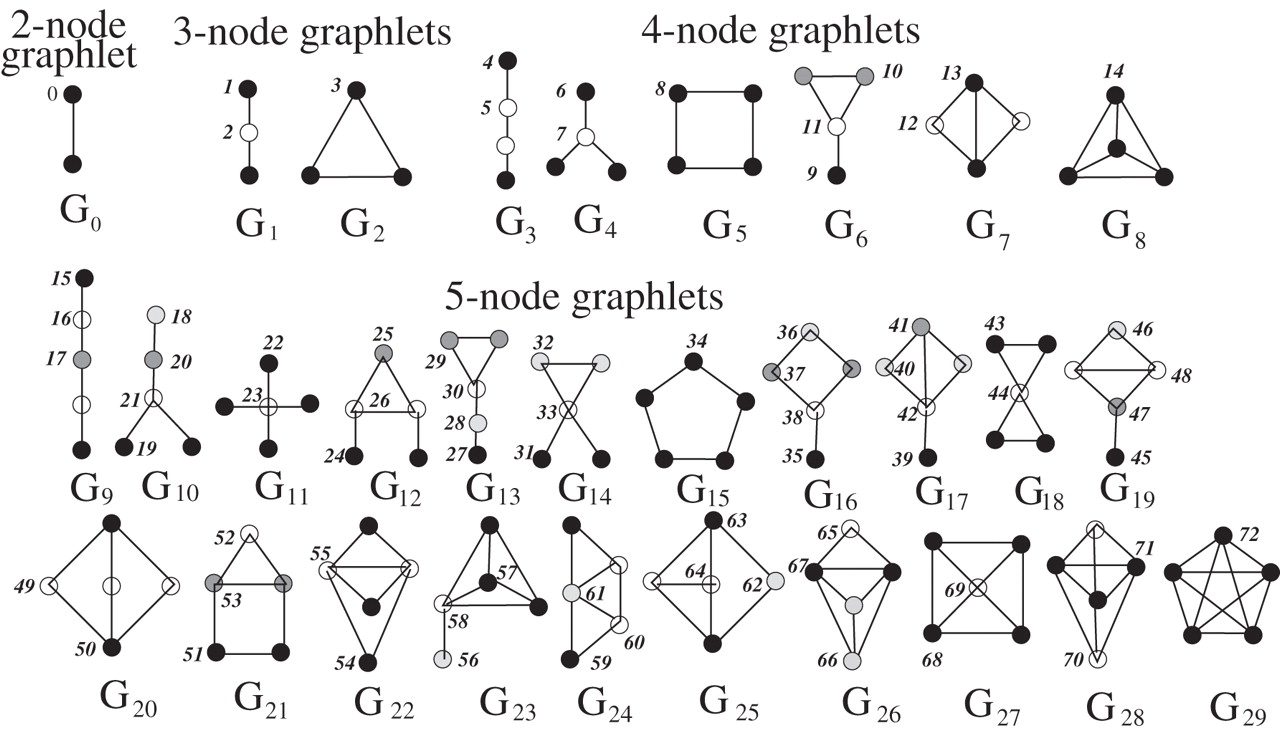
\includegraphics[scale=0.36]{images/graphlets.jpg}
\caption[Graphlets for sizes of 2, 3, 4 and 5 nodes]{Graphlets for sizes of 2, 3, 4 and 5 nodes. They are ordered in
groups according to the number of nodes they contain. These are the graphlets that are counted when computing
the GDV and GCV metrics. The node labels represent unique automorphism orbits. Source: \cite{milenkoviae2008uncovering} }
\label{fig:graphlets}
\end{figure}

Graphlets are small connected non-isomorphic\footnote{No two graphs from the set are the same.} induced\footnote{An induced subgraph is a subset of the vertices of a graph $G$ together with any edges whose endpoints are in the subset.} subgraphs of a graph. See definitions \ref{def:non_iso} and \ref{def:induced} for what non-isomorphic and induced graphs are. Figure \ref{fig:graphlets} shows all the graphlets of 2,3,4 and 5 nodes. They have been previously used by Nata\v{s}a et al. \cite{milenkoviae2008uncovering,prvzulj2007biological} for developing signatures such as the Graphlet Degree Vector (GDV) that quantify the local topological structure around a node.

For a given graph $G$, the \emph{Graphlet Frequency Vector} (GFV) can be calculated by
counting the number of distinct graphlets of each type found in $G$.
From here, we normalise the GFV against the total number of graphlets in $G$ to
calculate the \emph{Relative Graphlet Frequency Vector} (RGFV).

\begin{mydef}
\label{def:rgfv}
Let $G_i$ be the total number of graphlet of type $i$ in graph $G$. Then the Relative Graphlet Frequency Vector (RGFV) is defined as:

\begin{equation}
 GFV(G) = \left(F_1(G), F_2(G), ... F_{29}(G)\right)
\end{equation}
where 
$$ F_i(G) = -\log\left(\frac{G_i}{\sum_{i=1}^{n}G_i}\right) $$

\end{mydef}


\begin{figure}[h]
  \centering
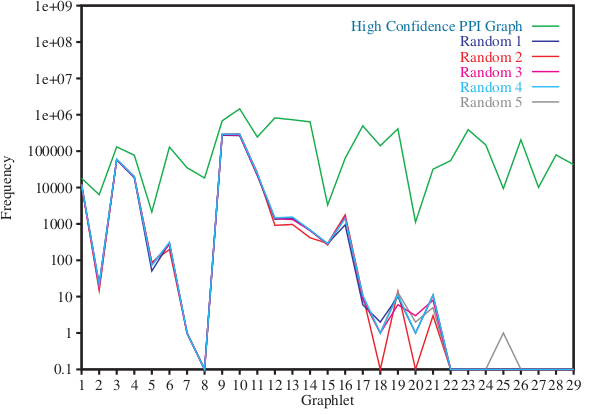
\includegraphics[scale=0.9]{images/gdv-er-interactome.png}
\caption[Graphlet Frequency Vectors for S. cerevisiae PPI network]{Example of \emph{Graphlet Frequency Vectors} for several random graphlets of a PPI network of
\emph{S. cerevisiae} (baker's yeast). As one can see from the plot, the GFV
signature of the real network is considerably different from the ones of the
random networks. The random networks have been generated using the Erd\H{o}s-R\'{e}nyi
method. Source: \cite{prvzulj2004modeling}}
\label{fig:gdv_er}
\end{figure}

\subsection{Relative Graphlet Frequency Distance}
\label{sec:rgfd}

Using the Graphlet frequencies that have been previously defined, we can now
compute a measure of disparity between two graphs by taking pairs of
graphlet frequencies for each type and then summing their absolute difference.
This is called the \emph{Relative Graphlet Frequency Distance} (RGFD). It is formally defined as follows:

\begin{mydef}
\label{def:rgfd}
Let $G$ and $H$ be two graphs and let \(F_i(G)\) and
\(F_i(H)\) be the frequency of the $i^{th}$ graphlet in $G$ and $H$ respectively. The Relative Graphlet Frequency Distance is then defined as:
$$  D = \sum_{i=1}^{n}| F_i(G) - F_i(H) | $$
\end{mydef}


\subsection{Graphlet Degree Vectors}
\label{sec:gdv}

In order to explain what a \emph{Graphlet Degree Vector} is, we first need to come back to automorphism orbits. For a node $x$, its automorphism orbit is the set of nodes similar to $x$ in the graph that could be interchanged with it in an automorphism operation. See definition \ref{def:automorphism_orbit} on page \pageref{def:automorphism_orbit} for a formal definition of the automorphism orbits. 


Figure \ref{fig:graphlets} shows the automorphism orbits for all the nodes in each of the 29 different graphlets. The different automorphism orbits are labelled with numbers ranging from 0 to 72, and the nodes in each graphlet are coloured according to which automorphism orbit it belongs to. Now that we have defined automorphism orbits, we can give a full definition of the \emph{Graphlet Degree Vector} of a node:

\begin{mydef}
For a node $x$ in a graph $G$, its Graphlet Degree Vector or GDV is a vector of $73$ coordinates, where each coordinate $i$ measures the number of graphlets that touch node $x$ at automorphism orbit $i$.
\end{mydef}

The GDV generalises the degree of a node, which counts the number of edges it touches, into the vector of graphlet degrees, which counts the number of graphlets that the node touches at a particular automorphism orbit. The resulting signature describes the local topology of the node neighbourhood up until a distance of 4 \cite{milenkoviae2008uncovering}.

For a given node $x$ in a graph $G$, we denote by $x_i$ the $i^{th}$ coordinate of the GDV vector of $x$. That is, $x_i$ is the number of times $x$ is touched at orbit $i$. 

\begin{mydef}
The distance $D_i(x,y)$ between the $i^{th}$ automorphism orbits of nodes $x$ and $y$ is defined as: 

\[D_i(x,y)=w_i \frac{|\log(x_i+1)-\log(y_i+1)|}{\log(\max(x_i,y_i)+2)}\]
where $w_i \in [0,1]$ are weights that normalise orbit dependency \emph{\cite{milenkoviae2008uncovering}}.
\end{mydef}

The logarithm function is used because the $i^{th}$ coordinates of the signature vectors of two nodes can differ by several order of magnitude and we do not want the distance measure to be dominated by the larger values \cite{milenkoviae2008uncovering}. We also add 1 to $u_i$ and $v_i$ in order to prevent the logarithm from going to $-\infty$. We add 2 in the denominator of the formula in order to prevent it from being infinite or 0 \cite{milenkoviae2008uncovering}.


\begin{mydef}
\label{def_gdv_dist}
Given two GDVs of nodes $x$ and $y$, the distance $D(x,y)$ between the GDVs of $x$ and $y$ is defined as:
$$D(x,y)= \frac{\sum_{i=0}^{72}D_i}{\sum_{i=0}^{72}w_i} $$ 
\end{mydef}

The distance measure given in definition \ref{def_gdv_dist} is in the $[0,1]$ range, where a distance of $0$ means that the two GDVs are identical. 

\begin{mydef}
\label{def_gdv_sim}
The signature similarity between nodes $x$ and $y$ is defined as:
$$S(x,y) = 1 - D(x,y) $$ 
\end{mydef}

The signature similarity gives a measure of how similar the topological structure around two nodes is. This is very useful because it can be easily applied to practical problems. For instance, it has been shown that the function of a protein can be predicted from its interactions \cite{letovsky2003predicting}. Therefore, if a protein $x$ is known to have a particular function and one would like to annotate a different, unknown protein $y$, one can transfer the function from $x$ to $y$ if their GDV signature similarity is high.

\subsection{Graphlet Degree Distributions}
\label{sec:gdd}

The Degree Distribution of a network calculates the number of nodes touching $k$
edges for each value of $k$. However, we can generalise this concept by looking
at the 73 automorphism orbits (see figure \ref{fig:graphlets}) and counting the
number of nodes that touch a particular graphlet at a particular orbit. Finally,
we get a spectrum of 73 \emph{Graphlet Degree Distributions (GDDs)} measuring
local properties of a network. 

We are now trying to compare the spectrum of 73 Graphlet Degree Distributions
belonging to a graph $G$ to the ones corresponding to another graph $H$. There
might be several ways to perform this, but we will present the method used by
N. Pr\v{z}ulj et al. in 2006 \cite{prvzulj2007biological}. 

\begin{mydef}

Let $G$ be a graph and let \( d_G^j(k) \) be a sample distribution of the
number of nodes in $G$ touching orbit $j$ ($j$ = $1-73$) $k$ times. \( d_G^j
\) represents the $j^{th}$ graphlet degree distribution (GDD). The scaled $j^{th}$ graphlet degree distribution $S_G^j(k)$ of $G$ is then defined as: 

$$ S_G^j(k) = \frac{d_G^j(k)}{k} $$

\end{mydef}


The reason for scaling \( d_G^j\) is because most of the information is retained in the lower
degrees, whereas the high degrees mostly contain
noise \cite{prvzulj2007biological}. Afterwards, the distribution is normalised
against its total area:

$$ T_G^j = \sum_{k=1}^{\infty}S_G^j(k) $$

giving the normalised distribution:

$$ N_G^j(k) = \frac{S_G^j(k)}{T_G^j}. $$

The reason why we are normalising the distribution is because a large
network would have a lot of nodes that potentially touch orbit $j$ and therefore a
large area under the curve. Normalising it would make large and small
biological networks comparable in terms of their GDD. 

\begin{mydef}
For two graphs $G$ and $H$ and an orbit $j$, we define the distance \( D^j(G,H) \) between their normalised $j^{th}$ distributions as:
$$ D^j(G,H) = \sqrt{\sum_{k=1}^{\infty}[N_G^j(k) - N_H^j(k)]^2} $$
\end{mydef}

The distance \( D^j(G,H) \) is between 0 and 1, where 0 means that $G$ and $H$ have
the same GDD for automorphism orbit $j$. Now that we have a measure of distance between two graphs $G$ and $H$, we need to invert the this distance in order to get the \emph{$j^{th}$ GDD agreement}:

\begin{mydef}

For two graphs $G$ and $H$ and an orbit $j$, we define the $j^{th}$ GDD agreement between their normalised $j^{th}$ distributions as:
$$ A^j(G, H) = 1 - D^j(G,H)$$
Moreover, the overall GDD agreement between the two
networks $G$ and $H$ is defined as the arithmetic mean of \( A^j(G,H) \) over all $j$:
 
$$ A(G,H) = \frac{1}{73}\sum_{j=0}^{72}A^j(G,H) $$  
\end{mydef}

The GDD agreement is like the GDV signature similarity of two nodes $x$ and $y$, but this time for the overall graphs $G$ and $H$. This measure can be used to compare different networks or even evaluate which random graphs best model the real data.

\section{Random graphs}

Random graphs are graphs that are usually generated using a random process. They are used in data analysis for comparing or aligning them against real networks. They can model the behaviour of real-world networks, such as the World Wide Web or PPI networks. Random graph models have been successfully used in various biological settings, such as: Network motifs \cite{milo2002network}, De-noising of protein-protein interaction network data \cite{kuchaiev2009geometric} or guiding biological experiments \cite{lappe2003unraveling}. In the next sections we will present several types of random graphs along with their properties.

\subsection{Erd\H{o}s-R\'{e}nyi graphs}

The work on random graph models started from the influential publications of
Erd\H{o}s and R\'{e}nyi in the 1950s and 1960s. Edgar Gilbert also published a similar
model later on. Erd\H{o}s and R\'{e}nyi described the \(G_{n,m}\)
model \cite{erdHos1959random}, while Gilbert described the \(G_{n,p}\)
model \cite{gilbert1959random}. These two methods can be described as
follows: 
\begin{itemize}
 \item[\(\mathbf{G_{n,p}}\)]: We start with $n$ disconnected nodes and a given
probability $p$. We then go through every pair of nodes and connect them with
probability $p$.
 \item[\(\mathbf{G_{n,m}}\)]: We start with $n$ disconnected nodes and a target number of edges $m$. Afterwards, we randomly select $m$ pairs of nodes and connect them.
\end{itemize}

Although these networks are very easy to generate, it was later found
that real networks have a structure that is different from the
Erd\H{o}s-R\'{e}nyi graphs. More precisely, they have a different degree distribution and a low clustering coefficient. On the other hand, some real networks have a power-law degree distribution. For the Erd\H{o}s-R\'{e}nyi $ G_{n,p} $ graph, the degree distribution is binomial:

\begin{equation}
 P(k) = {n-1 \choose k} p^k (1-p)^{n-1-k}
\end{equation}
which can be approximated with a Poisson distribution for a large $n$:

\begin{equation}
 P(k) = \frac{z^k * e^{-z}}{k!}
\end{equation}

\begin{figure}[H]
\begin{center}
\begin{subfigure}{.3\textwidth}
  \centering
  \begin{tikzpicture}[scale=1.0,auto,swap]

    % define the round nodes
    \foreach \pos/\name/\label in {
	{(0.000, 2.000)//0a},
	{(0.813, 1.827)//1a},
	{(1.486, 1.338)//2a},
	{(1.902, 0.618)//3a},
	{(1.989, -0.209)//4a},
	{(1.732, -1.000)//5a},
	{(1.176, -1.618)//6a},
	{(0.416, -1.956)//7a},
	{(-0.416, -1.956)//8a},
	{(-1.176, -1.618)//9a},
	{(-1.732, -1.000)//10a},
	{(-1.989, -0.209)//11a},
	{(-1.902, 0.618)//12a},
	{(-1.486, 1.338)//13a},
	{(-0.813, 1.827)//14a}}
      \node[vertex2] (\label) at \pos {$\name$} ;
	  


  \end{tikzpicture}
  \caption{$p = 0$}
  \label{fig:p00}
\end{subfigure}%
\begin{subfigure}{.3\textwidth}
  \centering
  \begin{tikzpicture}[scale=1.0,auto,swap]

    % define the round nodes
    \foreach \pos/\name/\label in {
	{(0.000, 2.000)//0a},
	{(0.813, 1.827)//1a},
	{(1.486, 1.338)//2a},
	{(1.902, 0.618)//3a},
	{(1.989, -0.209)//4a},
	{(1.732, -1.000)//5a},
	{(1.176, -1.618)//6a},
	{(0.416, -1.956)//7a},
	{(-0.416, -1.956)//8a},
	{(-1.176, -1.618)//9a},
	{(-1.732, -1.000)//10a},
	{(-1.989, -0.209)//11a},
	{(-1.902, 0.618)//12a},
	{(-1.486, 1.338)//13a},
	{(-0.813, 1.827)//14a}}
      \node[vertex2] (\label) at \pos {$\name$} ;
	      
    %neighbouring graph
	  
    \path[hi, line width=1.0]  (7a)  -- (2a);
    \path[hi, line width=1.0]  (8a)  -- (1a);
    \path[hi, line width=1.0]  (8a)  -- (3a);
    \path[hi, line width=1.0]  (9a)  -- (1a);
    \path[hi, line width=1.0]  (9a)  -- (4a);
    \path[hi, line width=1.0]  (10a)  -- (5a);
    \path[hi, line width=1.0]  (13a)  -- (1a);
    \path[hi, line width=1.0]  (13a)  -- (12a);
    \path[hi, line width=1.0]  (14a)  -- (6a);
    \path[hi, line width=1.0]  (14a)  -- (7a);
    \path[hi, line width=1.0]  (14a)  -- (11a);


  \end{tikzpicture}
  \caption{$p = 0.1$}
  \label{fig:p01}
\end{subfigure}%
\begin{subfigure}{.3\textwidth}
  \centering
  \begin{tikzpicture}[scale=1.0,auto,swap]

    % define the round nodes
    \foreach \pos/\name/\label in {
	{(0.000, 2.000)//0a},
	{(0.813, 1.827)//1a},
	{(1.486, 1.338)//2a},
	{(1.902, 0.618)//3a},
	{(1.989, -0.209)//4a},
	{(1.732, -1.000)//5a},
	{(1.176, -1.618)//6a},
	{(0.416, -1.956)//7a},
	{(-0.416, -1.956)//8a},
	{(-1.176, -1.618)//9a},
	{(-1.732, -1.000)//10a},
	{(-1.989, -0.209)//11a},
	{(-1.902, 0.618)//12a},
	{(-1.486, 1.338)//13a},
	{(-0.813, 1.827)//14a}}
      \node[vertex2] (\label) at \pos {$\name$} ;
	      
    %neighbouring graph
	  
    \path[hi, line width=1.0]  (2a)  -- (1a);
    \path[hi, line width=1.0]  (4a)  -- (2a);
    \path[hi, line width=1.0]  (5a)  -- (4a);
    \path[hi, line width=1.0]  (6a)  -- (2a);
    \path[hi, line width=1.0]  (8a)  -- (0a);
    \path[hi, line width=1.0]  (8a)  -- (3a);
    \path[hi, line width=1.0]  (8a)  -- (6a);
    \path[hi, line width=1.0]  (8a)  -- (7a);
    \path[hi, line width=1.0]  (9a)  -- (2a);
    \path[hi, line width=1.0]  (10a)  -- (2a);
    \path[hi, line width=1.0]  (10a)  -- (5a);
    \path[hi, line width=1.0]  (11a)  -- (6a);
    \path[hi, line width=1.0]  (11a)  -- (8a);
    \path[hi, line width=1.0]  (12a)  -- (1a);
    \path[hi, line width=1.0]  (12a)  -- (3a);
    \path[hi, line width=1.0]  (13a)  -- (4a);
    \path[hi, line width=1.0]  (14a)  -- (0a);
    \path[hi, line width=1.0]  (14a)  -- (1a);
    \path[hi, line width=1.0]  (14a)  -- (2a);
    \path[hi, line width=1.0]  (14a)  -- (4a);
    \path[hi, line width=1.0]  (14a)  -- (9a);
    \path[hi, line width=1.0]  (14a)  -- (11a);
    \path[hi, line width=1.0]  (14a)  -- (13a);



  \end{tikzpicture}
  \caption{$p = 0.2$}
  \label{fig:p02}
\end{subfigure}%
\end{center}
\caption[Erd\H{o}s-R\'{e}nyi graphs]{Example of three Erd\H{o}s-R\'{e}nyi random graphs generated using the
\(G_{n,p}\) method. The three different graphs differ with respect to the
probability $p$ of connecting one pair of nodes: (\subref{fig:p00}) $p = 0$ -- the graph is completely
disconnected. (\subref{fig:p01}) $p = 0.1$ -- the graph is sparsely connected because the probability $p$ is low
(\subref{fig:p02}) $p = 0.2$ -- the graph becomes more dense because of the increase of $p$ .}
\label{fig:erdos_renyi_graphs}
\end{figure}


\subsection{Erd\H{o}s-R\'{e}nyi with preserved degree distribution}
\label{er-dd}

As we have previously seen, the degree distribution of an Erd\H{o}s-R\'{e}nyi graph
does not match the real data. We will now present a method for constructing an
Erd\H{o}s-R\'{e}nyi network that preserves the degree distribution of a real network. 

We start with $n$ disconnected nodes. Each node is assigned a number of stubs 
according to the degree distribution of the real network that is being
modelled. A stub is simply a slot belonging to a particular node from where an edge can 
be connected. Afterwards, edges are created only between random pairs of nodes with
available stubs. After an edge is created, the number of stubs left available
at the nodes that were just connected is decreased by one. Moreover, edges
between one node and itself are not allowed.

This "stubs method" allows us to create Erd\H{o}s-R\'{e}nyi networks that have a power-law
degree distribution and a small average path length. Unfortunately, they still
have a low clustering coefficient.

\subsection{Scale-free networks}

\begin{figure}
  \centering
  \begin{subfigure}[b]{0.4\textwidth}
    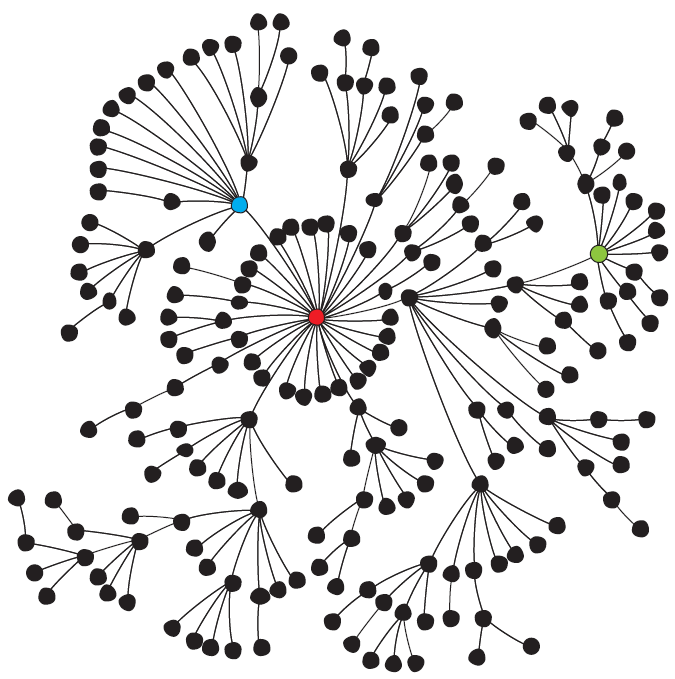
\includegraphics[width=\textwidth]{images/scale-free-network.png}
    \caption[Scale free network]{Example of a scale-free network. Note the large
    number of nodes of small degree at the periphery of the network, while the
    number of hub nodes is very small.}
    \label{fig:scale_free_network}  
  \end{subfigure}
  ~ %add desired spacing between images, e. g. ~, \quad, \qquad etc.
    %(or a blank line to force the subfigure onto a new line)
  \begin{subfigure}[b]{0.5\textwidth}
    \centering
    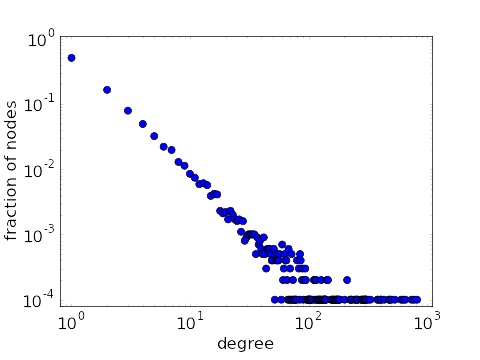
\includegraphics[width=\textwidth]{images/deg_dist_scale_free.png}
    \caption{The power-law degree distribution of a scale-free network. As the degree of
the nodes gets larger, the fraction of nodes decreases exponentially. Notice
the logarithmic scale on the Y axis. It has been observed that many real
networks exhibit a power-law degree distribution \cite{jeong2000large,faloutsos1999power,adamic2001search}.}
    \label{fig:degree_distribution}    
   \end{subfigure}
   \caption[Power-law degree distribution of a scale free network]{Scale-free network (\subref{fig:scale_free_network}) and power-law degree distribution (\subref{fig:degree_distribution})}
   \label{fig:scale_free} 
\end{figure}


Scale-free networks are networks that normally exhibit a power-law degree
distribution (see fig \ref{fig:scale_free}). That is, $ P(k) = k^{-\gamma} $,
where $P(k)$ is the fraction of nodes having degree $k$. It is currently believed that many networks such as the
World Wide Web, social networks or biological networks exhibit scale-free properties with a power-law degree distribution.

\subsubsection{Barab\'{a}si-Albert model}

There are several proposed ways in which scale-free networks can be
generated. The Barab\'{a}si-Albert model is one such technique that uses the
\emph{preferential attachment} mechanism, with which nodes of high degree have
a high probability of receiving even more connections. 

In order to construct a network using the Barab\'{a}si-Albert method, we start with
an initial connected network of $ m_0  $ nodes. New nodes are consecutively
added to the network one at a time. Each one of them is connected to $ m \le m_0 
$ target nodes with a probability that is proportional to the degree of the
target nodes. Formally, the probability $ p_i $ that the new node is connected
to node $i$ is:

\begin{equation}
 p_i = \frac{k_i}{\sum_{j}k_j}
\end{equation}

where $ k_i $ is the degree of node $i$, while the sum is over all the
nodes $j$ that already existed in the network when the new node is added. Because
of the preferential mechanism, heavily linked nodes (also called hub nodes)
tend to quickly accumulate links, whereas nodes with a low degree are unlikely
to be chosen. It has also been shown that the starting network heavily
influences the properties of the resulting network \cite{hormozdiari2007not}.

\subsection{Geometric graphs}

Geometric graphs are generated by fixing a certain metric space and using
metrics such as geometric distance or radius to connect edges together. A
metric space is a space that has a distance norm associated to it such as: the
Euclidean distance, Chessboard distance or Manhattan distance.

Such a network is generated in the following manner:
\begin{enumerate}
 \item Choose a metric space and place nodes within the space using a uniform
random distribution.
 \item If any nodes are within distance $d$ from each other, then connect them
with an edge.
 \item $d$ needs to be chosen so that the end number of edges matches the network
that is modelled.
\end{enumerate}

\begin{figure}[H]
  \centering
  \begin{subfigure}[b]{0.45\textwidth}
    \centering
    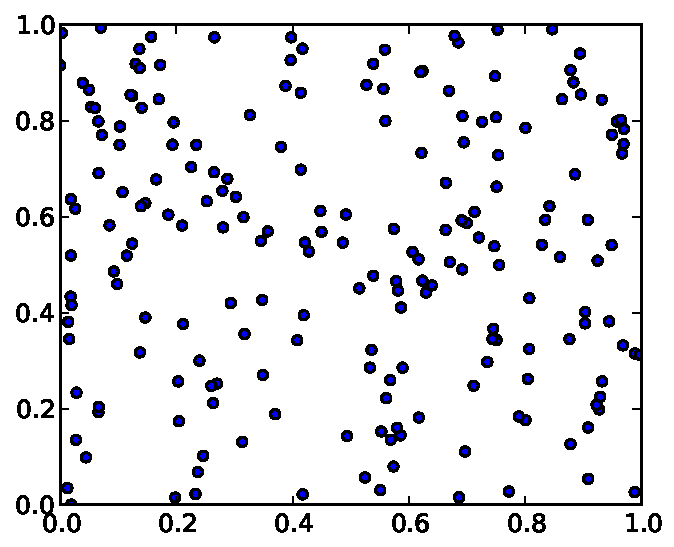
\includegraphics[scale=0.65]{../code/final_results/geometric_graphs/geo1.pdf}
    \caption{$d = 0.0$}
    \label{fig:geo1}  
  \end{subfigure}
  ~ %add desired spacing between images, e. g. ~, \quad, \qquad etc.
    %(or a blank line to force the subfigure onto a new line)
  \begin{subfigure}[b]{0.45\textwidth}
    \centering
    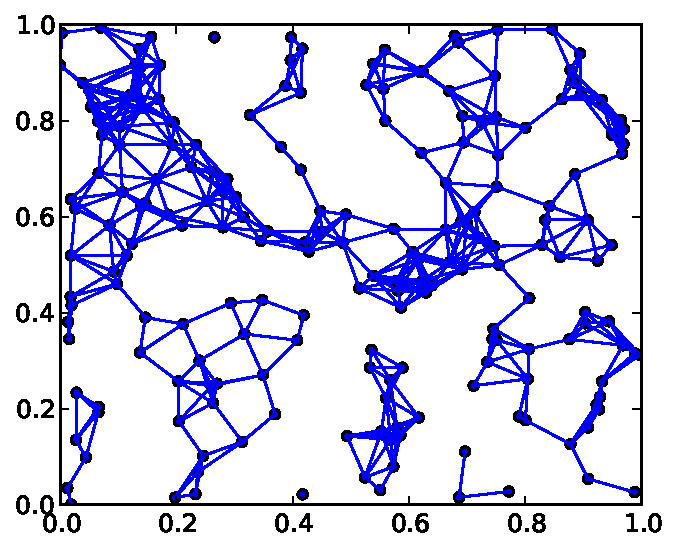
\includegraphics[scale=0.65]{../code/final_results/geometric_graphs/geo2.pdf}
    \caption{$d = 0.1$}
    \label{fig:geo2}    
   \end{subfigure}
    ~ %add desired spacing between images, e. g. ~, \quad, \qquad etc.
    %(or a blank line to force the subfigure onto a new line)
  \begin{subfigure}[b]{0.45\textwidth}
    \centering
    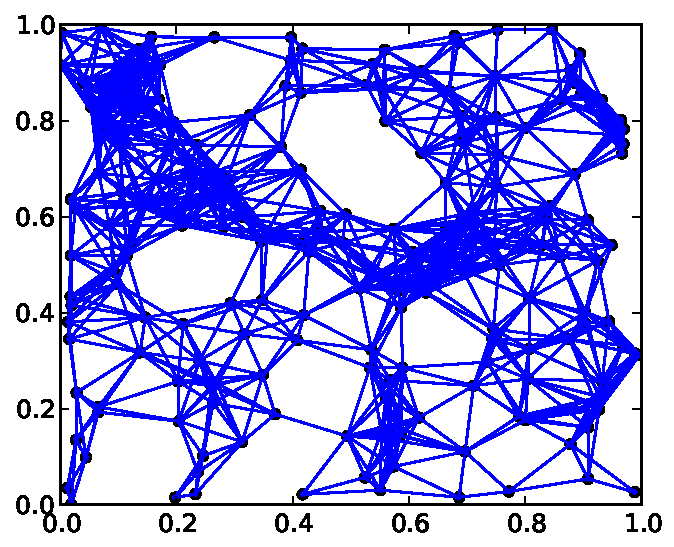
\includegraphics[scale=0.65]{../code/final_results/geometric_graphs/geo3.pdf}
    \caption{$d = 0.15$}
    \label{fig:geo3}    
   \end{subfigure}
    ~ %add desired spacing between images, e. g. ~, \quad, \qquad etc.
    %(or a blank line to force the subfigure onto a new line)
  \begin{subfigure}[b]{0.45\textwidth}
    \centering
    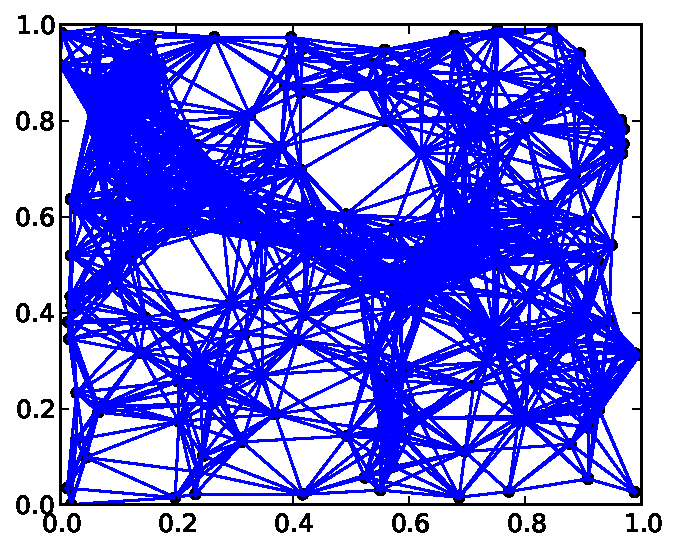
\includegraphics[scale=0.65]{../code/final_results/geometric_graphs/geo4.pdf}
    \caption{$d = 0.2$}
    \label{fig:geo4}    
   \end{subfigure}
   \caption[Geometric random graphs]{Geometric random networks built using different values for the distance parameter $d$, starting from
$d = 0$. Initially, nodes are distributed randomly across a metric space. When $d = 0$ in graph (\subref{fig:geo1}), the nodes are all disconnected from each other. As $d$ increases in graphs (\subref{fig:geo2} -- \subref{fig:geo4}), the number of connections in the network also increases proportionally. When using a Geometric network to model a real network, one would normally use a value of $d$ that would yield a similar number of edges as the real network.}
   \label{fig:geometric} 
\end{figure}


\subsection{Stickiness index-based graphs}

Pr\v{z}ulj et al. have proposed in 2006 a simple random
graph model that inserts a connection according to the degree or \emph{stickiness}
of the nodes involved \cite{prvzulj2006modelling}. This model has been inspired
from analysing protein-protein interactions and is based on two assumptions:
\begin{enumerate}
 \item A node with a high degree or \emph{stickiness} represents a protein that has many binding domains and/or its binding domains are
commonly involved in interactions.
 \item A pair of proteins is more likely to interact, or share complementary
binding domains, if they both have a high \emph{stickiness}. On the other hand,
if one or both of them have a low \emph{stickiness} index, they are less likely to
interact. Thus, the product of their stickiness values can be used as the
probability of connecting the nodes.
\end{enumerate}

Considering the above assumptions, a stickiness based random graph can be
constructed as follows:
\begin{enumerate}
 \item We start with a network of $n$ nodes each having a degree $ deg_i $
sampled from a degree distribution of our choice
 \item For each node $i$, we compute the stickiness index $
\theta_i=deg_i/\sqrt{\sum_{j=1}^{N}deg_j}. $ Note that $ 0 \leq \theta_i \leq 1$
 \item For each pair of nodes $(i,j)$, we connect them with probability $
\theta_i \theta_j $
\end{enumerate}


\subsection{Random graph Comparisons}

Now that we have presented a few commonly used random graph generating methods, we would like to compare them in terms of their underlying properties. As can be clearly seen in table \ref{tab:network_comparison}, real networks
normally have a power-law degree distribution, high clustering coefficient and
a small average path length. In terms of degree distribution, only Erd\H{o}s-R\'{e}nyi
(with a preserved degree distribution), Barab\'{a}si-Albert and Stickiness-based
random networks have a power-law degree distribution, which is found in real
networks. However, it must be noted that although most of the real networks
have a power-law degree distribution, this subject is still a matter of research. For
example, it has been shown that the Interactome network can be better modelled with
a Geometric network that has a Poisson degree distribution \cite{prvzulj2004modeling}.

On the other hand, only the Geometric and the Stickiness based models have a
high clustering coefficient. This is again something which has been observed in
most of the real networks such as social networks or biological networks.
Finally, most of the networks have a small average path length. It can
therefore be noted that the Stickiness-based network is the most successful
at modeling real-world phenomena with respect to these three properties.
However, there might be other network properties, such as various node
centralities \cite{newman2009networks} or \emph{Relative Graphlet Frequency
Agreement}, with can also be employed to
assess the suitability of the random networks. Identifying which of these 
properties can best compare various types of networks is still an open problem in
Network Analysis.

\definecolor{blue3}{HTML}{86B7FC} % med blue
\definecolor{blue1}{HTML}{B5F1FF} % light blue
\definecolor{blue2}{HTML}{E0F9FF} % very light blue

\definecolor{darkgreen}{HTML}{000000} % dark green

\rowcolors{1}{blue1}{blue2}

\begin{table}
  \centering
  Comparison of real networks versus randomly generated networks 
  \begin{tabular}{ | l | c | c | c |  }
%     \hlinede
    \cellcolor{blue3} Model & \cellcolor{blue3} Degree Distribution &
  \cellcolor{blue3} Clustering coefficient & \cellcolor{blue3} Average path
length \\
    \hline
    Real networks & \textcolor{darkgreen}{Power-law} &
  \textcolor{darkgreen}{High} & \textcolor{darkgreen}{Small}\\
    \hline
    Erd\H{o}s-R\'{e}nyi & \textcolor{red}{Poisson} & \textcolor{red}{Low} &
  \textcolor{red}{Large (for small p)} \\
    \hline
    Erd\H{o}s-R\'{e}nyi - DD & \textcolor{darkgreen}{Power-law} &
  \textcolor{red}{Low} & \textcolor{darkgreen}{Small} \\
    \hline
    Barab\'{a}si-Albert & \textcolor{darkgreen}{Power-law} &
  \textcolor{red}{Low} & \textcolor{darkgreen}{Small} \\
    \hline
    Geometric (uniform) & \textcolor{red}{Poisson} &
  \textcolor{darkgreen}{High} & \textcolor{darkgreen}{Small} \\
    \hline
    Stickiness based & \textcolor{darkgreen}{Power-law} &
  \textcolor{darkgreen}{High} & \textcolor{darkgreen}{Small} \\
    \hline
  \end{tabular}
  \caption{As one can observe from the table above, some of the models
such as Erd\H{o}s-R\'{e}nyi are not suitable for modeling real networks according to
these metrics. On the other hand, the Stickiness based random graph satisfies all the three criteria. Nevertheless, other network properties might exist for which the Stickiness based random network does not match the corresponding real network.}
  \label{tab:network_comparison}
\end{table}

\section{Measuring Correlation}

In sections \ref{sec:rgfd} and \ref{sec:gdd} we presented two main methods for calculating
how closely two GDV vectors match: \emph{Relative Graphlet Frequency Distance}
 and \emph{Graphlet Degree Distribution Agreement}. However, other methods also exist that use correlation coefficients such as \emph{Pearson's product-movement correlation coefficient} or \emph{Spearman's rank correlation coefficient}. This section presents correlation techniques that can be used for GDV comparisons.

\subsection{Pearson's product-movement correlation coefficient}

Given two random variables $X$ and $Y$ from a population, \emph{Pearson's
correlation coefficient} or sometimes called \emph{Pearson's population
correlation coefficient} is defined as the ratio between the covariance of $X$
and $Y$ and the product of their standard deviation. It was introduced by Karl
Pearson and it is based on a similar idea by Francis Galton in 1880 \cite{stigler1989francis,lee1988thirteen}.

\begin{mydef}
The Pearson's product-movement correlation coefficient $ \rho_{X,Y} $ between random variables $X$ and $Y$ is defined as:

 $$ \rho_{X,Y} = \frac{\sigma_{XY}}{\sigma_X\sigma_Y} =
\frac{E[X-\mu_X]E[Y-\mu_Y]}{\sigma_X\sigma_Y}$$
where $ \sigma_{XY} $ is the covariance of $X$ and $Y$, while $\sigma_X $, $ \mu_X $ and $\sigma_Y $, $ \mu_Y $ are the standard deviation and the expectation of $X$ and $Y$ respectively.
\end{mydef}


Pearson's correlation coefficient can also be applied to a sample from a given
population, in which case it is called the \emph{sample Pearson's correlation
coefficient} and is commonly denoted by $r$. This can be calculated by using
sample estimators for the covariance and standard deviation in the formula
above. 

\begin{mydef}
The sample Pearson's product-movement correlation coefficient $ r_{X,Y} $ between population samples $X$ and $Y$ is defined as:

\begin{equation}
\label{pears_corr}
 r = \frac{\sum_{i=1}^{n}(X_i - \bar{X})(Y_i -
\bar{Y})}{\sqrt{\sum_{i=1}^{n}\left(X_i -
\bar{X}\right)^2}\sqrt{\sum_{i=1}^{n}\left(Y_i -
\bar{Y}\right)^2}} 
\end{equation}
where $ \sigma_{XY} $ is the covariance of $X$ and $Y$, while $\sigma_X $, $ \mu_X $ and $\sigma_Y $, $ \mu_Y $ are the standard deviation and the expectation of $X$ and $Y$ respectively.
\end{mydef}

The values of both the sample and the population variants of Pearson's
correlation coefficients are between -1 and 1. Sample data points that have 
exactly 1 or -1 as their correlation coefficient will lie on a straight line.
Moreover, Pearson's correlation coefficient is symmetric because: 

$$ \rho(X,Y) = \rho(Y,X) $$

where $\rho(X,Y)$ is defined as the correlation between random variables $X$ and $Y$.

\subsubsection{Pearson's distance}

Given a correlation coefficient $ \rho_{X,Y} $, a distance metric
called the \emph{Pearson's distance} can be derived as
follows \cite{fulekar2009bioinformatics}:

$$ d_{X,Y} = 1- \rho_{X,Y} $$

It should be noted that because Pearson's correlation coefficient lies between
-1 and 1, then the Pearson's distance will have a value between 0 and 2.

\subsubsection{Interpretation}

Several researchers have provided guidelines into how
to interpret the size of the correlation coefficient \cite{cohen1988statistical} 
(equation \ref{pears_corr}). However, interpretation is highly dependent on the context of the problem. For
example, a correlation of 0.8 might be low if one verifies physical laws using
measurements made with high-precision instruments, but it might be considered
high when applied to the analysis of social networks, because of underlying hidden
factors.

\subsection{Spearman's rank correlation coefficient}


% perf: pears (0.914, 0.000) spear (1.000, 0.000)
% spread: pears (0.086, 0.447) spear (0.114, 0.314)
% outliers: pears (0.557, 0.000) spear (0.810, 0.000)

\rowcolors{1}{}{}


\begin{figure}[h]
\begin{center}	
\begin{subfigure}{0.45\textwidth}
  \centering
  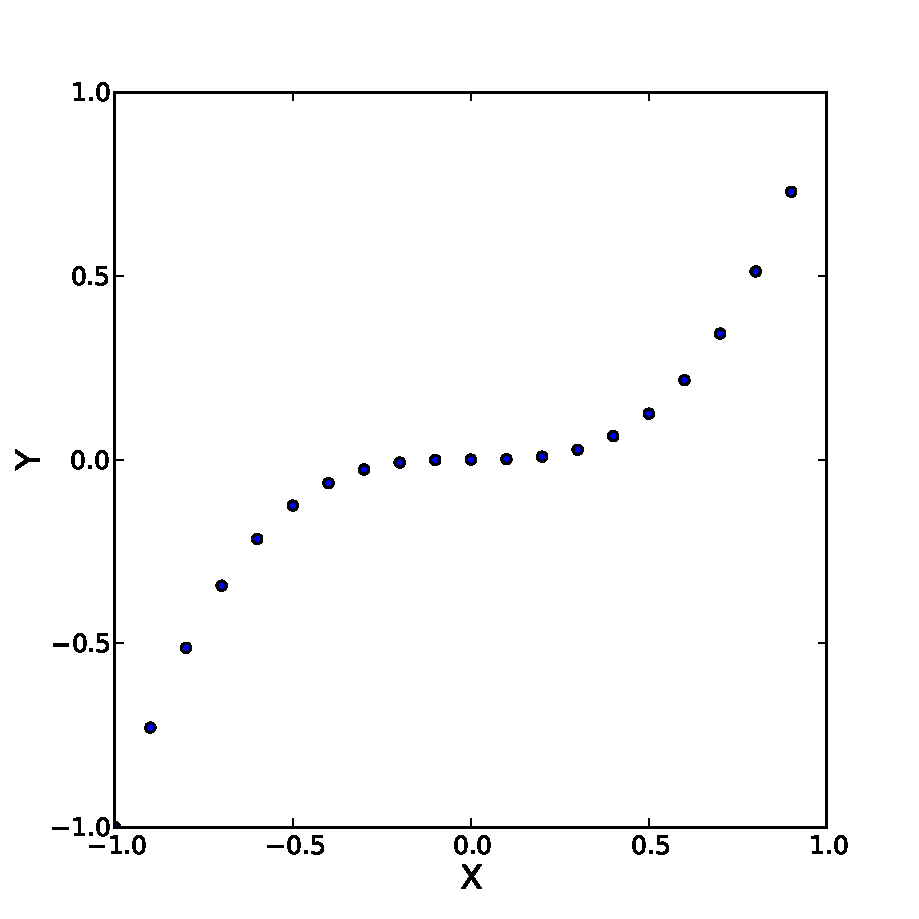
\includegraphics[width=\columnwidth]{../code/final_results/spearman_images/perfect.pdf}
  \caption{\begin{tabular}{r l}
 Pearson correlation: & 0.91\\
 p-value: & 0.0\\
 \hline
 Spearman correlation: & 1.0\\
 p-value: & 0.0
\end{tabular}}
  \label{fig:perf}
\end{subfigure}
\begin{subfigure}{0.45\textwidth}
  \centering
  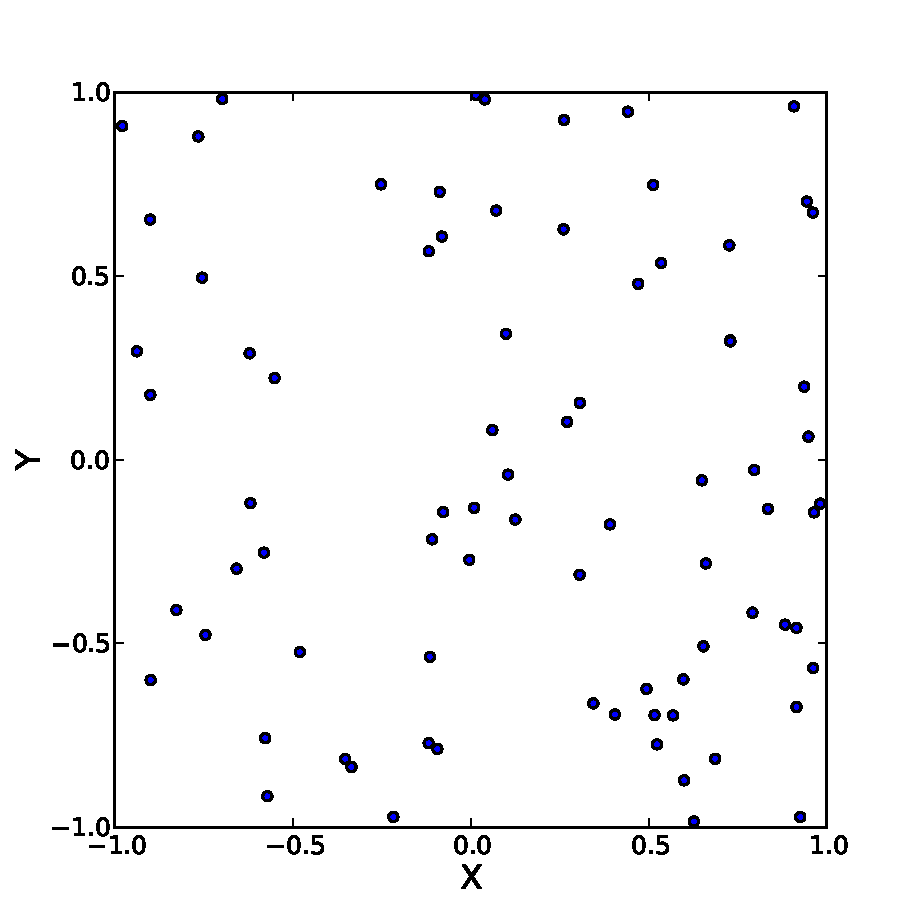
\includegraphics[width=\columnwidth]{../code/final_results/spearman_images/spread.pdf}
  \caption{\begin{tabular}{r l}
 Pearson correlation: & 0.08\\
 p-value: & 0.44\\
 \hline
 Spearman correlation: & 0.11\\
 p-value: & 0.31
\end{tabular}}  \label{fig:spread}
\end{subfigure}
\end{center}
\caption[Spearman's correlation coefficient -- perfectly correlated data vs random data ]{Spearman's correlation coefficient is measuring how well the
dependence between two variables $X$ and $Y$ can be modelled
using a monotonic function. A Spearman's correlation of 1 can result even
when the data points are not linear (subfigure \subref{fig:perf}), as long as they are monotonically related. For the same dataset, Pearson's correlation coefficient is 0.91. When the data points are evenly spread (subfigure \subref{fig:spread}), both the Pearson's and the Spearman's
correlation coefficients will be low ( 0.08 and
0.11 respectively) and their p-value will be high (0.44 and 0.31), suggesting that the correlation is not statistically significant.}
\end{figure}


\begin{figure}[h]
\begin{center}
\begin{subfigure}{0.45\textwidth}
  \centering
  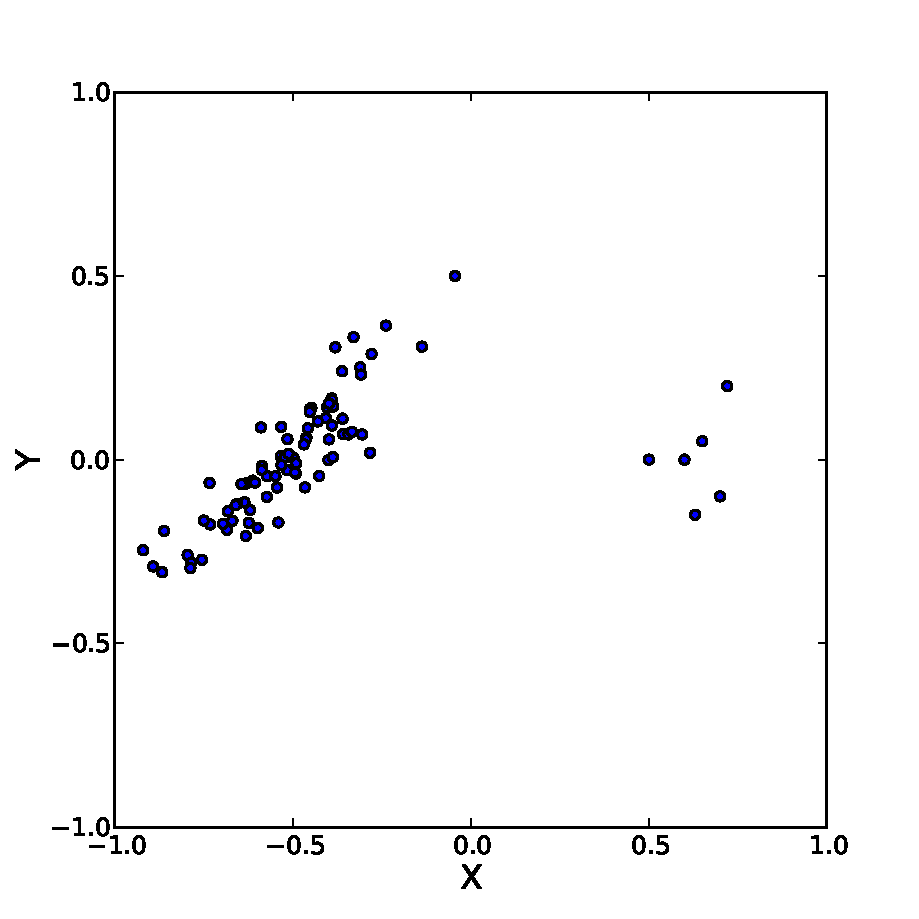
\includegraphics[width=\columnwidth]{../code/final_results/spearman_images/outliers.pdf}
  \caption{\begin{tabular}{r l}
 Pearson correlation: & 0.55\\
 p-value: & 0.0\\
 \hline
 Spearman correlation: & 0.81\\
 p-value: & 0.0
\end{tabular}}  \label{fig:outliers}
\end{subfigure}
\end{center}
\caption[Spearman's correlation coefficient -- outliers]{Spearman's rank correlation coefficient is less sensitive to outliers than Pearson's correlation coefficient, because each data point is first projected to its rank. For the above dataset, the Pearson's correlation coefficient is only 0.55, while Spearman's correlation coefficient is 0.81. Both correlations are statistically significant, since their p-values are below 0.05.}
\end{figure}


The Spearman's rank correlation coefficient or Spearman's rho, named after
Charles Spearman, is a non-parametric estimator of the statistical dependence of
two random variables \cite{lehman2005jmp}. It intuitively measures how well
the dependence between two variables can be measured using a monotonic function.
It is normally defined as follows:
\begin{mydef}
Let $X$ and $Y$ be two population samples and let $ x_i$ and $ y_i $ be the ranks of each of the data points in $X$ and $Y$. The Spearman's rank correlation coefficient is defined as the Pearson's correlation coefficient of the ranks $ x_i, y_i $ of the data points \emph{\cite{myers2010research}}.
\end{mydef}


\rowcolors{1}{blue1}{blue2}

\begin{table}
  \centering
  \begin{tabular}{ | c | c | c |}
    \hline
    \cellcolor{blue3} Variable $X_i$ & \cellcolor{blue3} Position & \cellcolor{blue3} Rank\\
    \hline
    0.3 & 1 & 1\\
    \hline
    0.6 & 2 & 2\\
    \hline
    1.2 & 4 & $ \frac{4+5}{2} $\\
    \hline
    1.2 & 5 & $ \frac{4+5}{2} $\\
    \hline
    0.8 & 3 & 3\\
    \hline
    1.9 & 6 & 1\\
    \hline
  \end{tabular}
  \caption{Computation of Spearman's ranks for a dataset of 6 samples. The data is initially sorted in ascending order. If the data point is
unique, then the rank is simply the position in the ordered list. Otherwise,
the rank is computed as the average of the positions of all the data points
with the same value.}
  \label{tab:ranks_table}
\end{table}

The calculation of the ranks is best illustrated in table \ref{tab:ranks_table}.
After the rank $ x_i, y_i $ of each data point is calculated,
the Spearman's correlation coefficient is computed using the formula for the Pearson's
correlation coefficient.


Spearman's correlation coefficient is considered non-parametric in the sense
that one does not need to know any prior on the $X$ and $Y$ random variables, as
it does not require knowledge (i.e.\ the parameters) of the joint probability
distribution of $X$ and $Y$.

\subsection{Computing the GDV correlation matrix of a network}
\label{pearsons_background}

We can use the Pearson's or Spearman's correlation coefficient previously
described to compute the \emph{GDV correlation matrix} for a given network in the
following manner:
\begin{enumerate}
 \item We compute the 73-element Graphlet Degree Vector (GDV) for every node in the
input network
 \item We then construct samples $ S_i, i\in {1,2,3, .. ,73} $
containing all the frequencies of the orbits of type $i$ found in the GDVs of
the nodes.
 \item We compute the Pearson's (or Spearman's) correlation coefficient of each
pair of samples $ (S_i, S_j) $ and we put them in the 73x73 correlation matrix $
C_{ij} $.
\end{enumerate}

The newly obtained graphlet correlation matrix will be symmetric with respect to 
the main diagonal, as Pearson's correlation coefficient is also symmetric. In
order to display such a matrix, we use a heat map, with blue representing a correlation of -1 and red representing a correlation of 1.

Given two matrices from two different networks $G$ and $H$, we then calculate
the \emph{Pearson's correlation matrix distance} between them by performing pairwise-subtractions of the elements. The \emph{Pearson's correlation matrix distance} is also referred to as the \emph{Graphlet correlation distance} in the literature \cite{yaverouglu2014revealing}.

\begin{mydef}
\label{def:gcd}
 Let $G$ and $H$ be two graphs and $G'$, $H'$ their Pearson's correlation matrices. The Pearson's correlation matrix distance or Graphlet correlation distance between $G$ and $H$ is then defined as:
 \begin{equation}
\label{pears_matrix_diff}
  D(G,H) = \sum_{i,j}\left(G'(i,j) - H'(i,j)\right)^2
\end{equation}
 
\end{mydef}

Note that the computed distance $D(G,H)$ is always greater than 0. We are now able to define the \emph{Graphlet Correlation Matrix Agreement}, which measures how similar two graphs are with respect to the GDV signatures.

\begin{mydef}
The \emph{Graphlet Correlation Matrix Agreement} between two graphs $G$ and $H$ is
defined as: 
 \begin{equation}
 Agreement = 1 - D(G,H)
 \end{equation}
\end{mydef}

One advantage of using the \emph{Graphlet Correlation Matrix Agreement} instead of the \emph{GDD agreement} previously defined is that it has been shown to be more robust to noise in the network data \cite{kuchaiev2009learning}.

\subsection{Hierarchical clustering}
\label{hier_clust}

When analysing the GDV correlation matrix of a network, we are interested to find out 
how graphlets group together with the rest of the graphlets according to their correlation. 
These groups of graphlets can be easily identified if we use \emph{hierarchical clustering}, 
which is a clustering method that builds a dendogram of the graphlets according to a distance function. 

The two main types of strategies for hierarchical clustering are:
\begin{itemize}
 \item Agglomerative (bottom-up): Each observation starts in its own cluster. At each step, the clusters with the smallest distance between each other are merged.  
 \item Divisive (top-down): All observations start in one cluster. At each step, the clusters are split recursively.
\end{itemize}

\subsubsection{Distance metric}
In order to perform \emph{hierarchical clustering}, a distance metric has to be defined. Some commonly-used metrics are:
\begin{itemize}
 \item Euclidean distance: $ \|a - b\|_2 = \sqrt{\sum_{i}(a_i - b_i)^2}$
 \item generalised p-norm: $ \|a - b\|_p = \left(\sum_{i}|a_i - b_i|^p\right)^\frac{1}{p}$
 \item Mahalanobis distance: $ \|a - b\| = \sqrt{(a - b)S^{-1}(a-b)}$, where $S$ is the covariance matrix
\end{itemize}


\subsubsection{Linkage criteria}

The linkage criteria defines the distance between the sets of data points as a function of the distances between the data points themselves. 

Some commonly used criteria for the linkage between two sets $A$ and $B$ are \cite{szekely2005hierarchical}:
\begin{itemize}
 \item Complete linkage clustering: $max \{d(a,b) | a \in A, b \in B\}$
 \item Single linkage clustering: $min \{d(a,b) | a \in A, b \in B\}$
 \item Average linkage clustering \cite{sokal1958statistical}: $max \{d(a,b) | a \in A, b \in B\}$
 \item Centroid linkage clustering: $ ||c_A - c_B|| $ where $c_A$ and $c_B$ are the centroids of clusters $A$ and $B$.
\end{itemize}


\section{Canonical Correlation Analysis}
\label{cca_background}

Canonical Correlation Analysis is a statistical method of analysing interdependence 
between two random variables $X$ and $Y$. The method was first introduced in 1936 by 
Harold Hotelling \cite{hotelling1936relations} and it has been used for 
analysing and interpreting data in various fields including 
Psychology \cite{cooley1971multivariate}, Marketing \cite{fader1990cross} and 
Operations Research \cite{pisharodi1991interset}.

Given two random variables $X$ and $Y$ and a set of vector weights $a_1$ and $b_1$, 
let $u_1 = Xb_1$ and $t_1 = Ya_1$. Canonical Correlation Analysis (CCA) aims to 
find the weights $a_1$ and $b_1$ such that the correlation $ \rho = r(t_1, u_1) $
is maximised. In this case, $u_1$ and $t_1$ are called the first canonical variates. 

The CCA process can be repeated again in order to find a second pair of canonical 
variates $u_2$ and $t_2$, with the additional condition that they are orthogonal to the first set 
of canonical variates $u_1$ and $t_1$. Thus, the second stage of the canonical correlation problem 
can be stated as follows:

Choose $a_2$,$b_2$ to maximise 
\begin{equation}
r(t_2, u_2) = r(Ya_2, Xb_2)
\end{equation}
such that 
$$r(t_1, t_2) = 0 \text{ and } r(u_1, u_2) = 0$$

This procedure can be repeatedly applied, although at each iteration the amount of correlation that we can achieve is decreasing. The reason for this is because each subsequent problem contains one extra orthogonality constraint compared to the previous one. The number of "stages" to the canonical correlation problem depends on the number of variables. 
If $p$ is the number of $X$ variables and $q$ is the number of $Y$ variables, then the maximum 
number of canonical variates that can be computed is $min(p,q)$.

\subsection{Derivation of Canonical Correlation Analysis}

We first define the correlation matrix $R$ as:

\rowcolors{1}{}{}

$$R = 
\begin{pmatrix}
R_{YY} & R_{YX} \\
R_{XY} & R_{XX} 
\end{pmatrix}
$$

where $R_{XY}$ is the correlation matrix between $X$ and $Y$, while $R_{XX}$ and $R_{YY}$ are the correlation matrices of $X$ and $Y$.  


We find that solving the problem in matrix form will in fact give the solution to all 
stages of the problem. Dropping the subscripts on variates $u = Xb$ and $t = Ya$, we restate the problem as follows:\\

Choose $a$, $b$ to maximise 

\begin{equation}
\label{cca_no_subscript}
r(t, u)=\frac{cov(t,u)}{\sqrt{var(t)var(u)}}
\end{equation}

The numerator of the objective function in equation (\ref{cca_no_subscript}) is simply given by:

$$Cov(t,u) = \frac{[t'u]}{n-1}=\frac{a'Y'Xb}{n-1} = a'R_{YX}b$$

By standardising $t$ and $u$, we effectively eliminate the denominator from the objective 
function in equation (\ref{cca_no_subscript}). Note that setting $ var(t) = 1 $ is equivalent to the following:
  
$$ var(t) = 1 $$
$$\implies \frac{[t't]}{n-1} = 1 $$
$$ \implies \frac{[a'Y'YA]}{n-1} = 1 $$
$$ \implies a'R_{YY}a = 1$$

Similarly, setting $var(u) = 1$ is the same as setting $b'R_{XX}b = 1$. Imposing these 
constraints, the problem becomes:\\

Choose $a$, $b$ to maximise 
$$a'R_{XX}b$$ 
subject to 
\begin{equation}
\label{cca_constraints}
a'R_{YY}a = 1 \text{ and } b'R_{XX}b = 1
\end{equation}

This constrained maximisation problem can be solved by using Lagrange multipliers and solving the first-order conditions. Using $\alpha/2$ and $\beta/2$ as Lagrange multipliers, the Lagrangian function is then given by:

\begin{equation}
 L = a'R_{YX}b - \frac{\alpha}{2}(a'R_{YY}a - 1) - \frac{\beta}{2}(b'R_{XX}b - 1) 
\end{equation}

Differentiating with respect to $a$ and $b$ and setting the results equal to zero gives the first-order necessary conditions:

\begin{equation}
\label{cca_foc1}
  \frac{\partial L}{\partial a} = 0 \implies R_{YX}b - \alpha R_{YY}a = 0
\end{equation}
\begin{equation}
\label{cca_foc2}
 \frac{\partial L}{\partial b} = 0 \implies R_{XY}a - \beta R_{XX}b = 0
\end{equation}

Taking the expression in equation (\ref{cca_foc1}) and premultiplying by $a'$ yields:

$$a'R_{YX}b - \alpha (a'R_{YY}a) = 0$$
which implies that $\alpha = r(t,u) $, the canonical correlation, because $a'R_{YY}a=1$ under the scaling constraints we have imposed for this problem. Similarly, taking equation (\ref{cca_foc2}) and premultiplying by $b'$ yields $\beta = r(t,u)$, which means that $\alpha = \beta$.

Now that the values of $\alpha$ and $\beta$ are known, we can substitute into equations (\ref{cca_foc1}) and (\ref{cca_foc2}) and solve the expressions for either $a$ or $b$.

Suppose we choose to solve for b. We use equation (\ref{cca_foc1}) to write $a$ as a function of $b$ as follows:

\begin{equation}
\label{cca_a}
  a = \frac{1}{r(t,u)}R^{-1}_{YY}R_{YX}b
\end{equation}

We then substitute the right-hand side of equation (\ref{cca_a}) above for $a$ in equation (\ref{cca_foc2}) and solve for $b$. The result is:

\begin{equation}
 R_{XY}\left( \frac{1}{r(t,u)}R^{-1}_{YY}R_{YX}b \right) = r(t,u)R_{XX}b
\end{equation}

Premultiplying by $R^{-1}_{XX}$ and mutiplying through by $r(t,u)$ gives:

\begin{equation}
  \label{cca_eigen_eq}
 [R^{-1}_{XX}R_{XY}R^{-1}_{YY}R_{YX}]b = r^2(t,u)b
\end{equation}

Equation (\ref{cca_eigen_eq}) is an eigenvector-eigenvalue problem. The vector $b$ is the first eigenvector of the matrix $R^{-1}_{XX}R_{XY}R^{-1}_{YY}R_{YX}$. The proportionality constant, which is the eigenvalue corresponding to $b$, is the squared canonical correlation $r^2(t,u)$. Although we will not prove this in the report, the structure of the canonical correlation problem ensures that the eigenvalues are both real and non-negative \cite{carroll1997mathematical}. 

We can now find $a$ by substituting $b$ into equation (\ref{cca_a}). We also find that $a$ is the first eigenvector of the matrix $R^{-1}_{YY}R_{YX}R^{-1}_{XX}R_{XY}$. The first eigenvalue is again the squared canonical correlation.

\subsection{Canonical Loadings}

To facilitate interpretation, it is helpful to look at canonical loadings, which are correlations between original variables and their corresponding canonical variates. The correlations between $X$ and $u$, which we denote $f$, are given by:

\begin{equation}
 f = \frac{1}{n-1}X'u = \frac{1}{n-1}X'(Xb) = R_{XX}b
\end{equation}
Similarly, the correlations between $Y$ and $t$, denoted $g$ are given by:
\begin{equation}
 g = \frac{1}{n-1}Y't = \frac{1}{n-1}Y'(Ya) = R_{YY}a
\end{equation}

\subsection{Canonical Cross-Loadings}

A slightly different concept is given by canonical cross-loadings, which are the correlations between original variables and the opposite canonical variates. The correlations between $X$ and $t$, which we denote $h$, are given by:

\begin{equation}
 h = \frac{1}{n-1}X't = \frac{1}{n-1}X'(Ya) = R_{XY}a
\end{equation}
The cross-loadings between $Y$ and $u$, denoted $j$ are given by:
\begin{equation}
 j = \frac{1}{n-1}Y'u = \frac{1}{n-1}Y'(Xb) = R_{YX}b
\end{equation}

In our project, when we present CCA results we only use canonical cross-loadings, because we are interested to find out how each element from one variate correlates with the elements from the opposite variate.

\subsection{Interpretation of Canonical Correlation Results}

The weights $a$ and $b$ that maximise the correlation $ \rho = corr(Xa, Yb) $ can be easily interpreted in the following manner:
\begin{itemize}
 \item If two values $a_i, b_j$ have the same sign it means that variables $X_i$, $Y_j$ are positively correlated. Similarly, if the values of $a_i, b_j$ have different signs then it means that the variables are negatively correlated. 
 \item A higher absolute value of $a_i$ and $b_j$ means that variables $X_i$, $Y_j$ show a stronger correlation. Similarly, if the absolute value of $a_i$ and $b_j$ is close to zero then it shows that variables $X_i$, $Y_j$ show a weak and insignificant correlation.
 \item If the weight vectors $a$ and $b$ are multiplied by scalars $\alpha$ and $\beta$ respectively, then the resulting correlation $ \rho' = corr(\alpha aX, \beta bY) $ is still the same as the original correlation between vectors $a$ and $b$, that is $ \rho = corr(Xa, Yb) $.
\end{itemize}

Note that in this report, when we say that two elements $x_i$ and $y_i$ of vectors $X$ and $Y$ correlate positively or have a positive correlation with respect to each other, it means that they have the same sign. Similarly, $x_i$ and $y_i$ will correlate negatively if they have opposite signs.

\section{Networks analysed}
\label{sec:networks_analysed}

Throughout the project we will be analysing several classes of networks:
\begin{itemize}
 \item Protein-Protein Interaction (PPI) networks
 \item Metabolic networks
 \item World Trade networks
%  \item Literature networks
\end{itemize}

 In order to perform Canonical Correlation Analysis, we have also used annotations, which are labels that offer information about each node in the graphs. For a country in the World Trade network (WTN), the annotations are financial indicators such as GDP per capita. On the other hand, for a protein in the PPI network these are properties such as "RNA transcription" or "energy production" that describe the function of the protein. Each of these networks and their annotations are described in detail in the following sections.

\subsection{Protein-Protein Interaction networks}
\label{sec:ppi_bck}

The Protein-Protein Interaction networks, or PPI networks are mainly represented by a graph where the nodes are proteins and the edges are interactions between proteins. These interactions are normally captured using technologies such as \emph{Yeast two-hybrid screening} \cite{young1998yeast} or \emph{affinity purification mass spectrometry} (AP-MS) \cite{brettner2012protein,wodak2013protein}.

The source of our PPI networks is the \emph{Biological General Repository for Interaction Datasets} (BioGRID). Throughout the project we have mainly focused on the Human PPI network, although some of our experiments have also been performed on the PPI networks of other model organisms such as C. elegans(worm), D. melanogaster(fruit fly), E. coli(bacteria), M. musculus(mouse) and S. cerevisiae(baker's yeast). We have done this in order to find out whether our results are consistent across a spectrum of networks from different species.

\subsubsection{Annotations}
\label{ppi_annotations}

In order to assign functional information to each protein in the PPI network, we have used \emph{Gene Ontology terms}, commonly called \emph{GO terms}. These are part of a large project called \emph{Gene Ontology} that aims to unify the representation of gene attributes across all species \cite{gene2008gene}. Moreover, we have also used two smaller annotation sets that only contained 13 and 14 functional terms respectively. The first one belongs to Christian von Mering et al. \cite{von2002comparative} and contains the following annotations:
\begin{multicols}{2}
\begin{itemize}
  \item Energy production
  \item Amino acid metabolism
  \item Other metabolism
  \item Translation
  \item Transcription
  \item Transcriptional control
  \item Protein fate
  \item Cellular organisation
  \item Transport and sensing
  \item Stress and defence
  \item Genome maintenance
  \item Cellular fate / organisation
  \item Uncharacterized
\end{itemize}
\end{multicols}

The second annotation file is from Charlie Boone \cite{costanzo2010genetic} and contains a slightly different annotation set:
\begin{multicols}{2}
\begin{itemize}
  \item Golgi endosome vacuole sorting
  \item Metabolism - mitochondria
  \item DNA replication
  \item Chromatin transcription
  \item Cell polarity morphogenesis
  \item Signalling stress response
  \item Chromatin  segmentation
  \item Protein folding
  \item ER Golgi traffic
  \item Nuclear cytoplasmic transport
  \item Cell cycle progression meiosis
  \item Protein degradation proteosome
  \item RNA processing
  \item Ribosome translation
\end{itemize}
\end{multicols}

Nevertheless, both annotation files label each proteins according to their function. Since these annotation sets are more compact\footnote{GO terms are in the order of thousands. A more compact version called GO Slim exists, which has around 100 different functional annotations.} than GO terms, we have found it easier to work with Boone's and von Mering's annotation files.

\rowcolors{1}{blue1}{blue2}

\begin{table}
  \centering
  Basic statistics of the Human PPI network\\
  \begin{tabular}{  c  c | c  c }
%     \hline
    Clustering coefficient & 0.125 & Number of nodes & 11099\\
    Connected components & 77 & Density & 0.001\\
    Network diameter & 13 & Heterogeneity & 1.945\\
    Average number of neighbours & 10.236 & Isolated nodes & 0\\
    Network centralisation & 0.046 & Number of self-loops & 0\\
    Shortest paths & 119,301,268 (96\%) & Multi-edge node pairs & 0\\
    Characteristic path length & 3.963 & Edges & 56806\\
%     \hline
  \end{tabular}
  \caption{Basic statistics for the Human PPI network. The Human PPI network has a large number of nodes (11099), a small clustering coefficient (0.125) and a large network diameter (13).}
  \label{tab:ppi_stats_table}
\end{table}

\subsection{Metabolic networks}
\label{sec:meta_bck}

A metabolic network is a set of chemical and metabolic processes that regulate physiological and biochemical properties of a cell. Therefore, these networks contain metabolic pathways and regulatory interactions that guide these processes. The source of our metabolic network data and annotations is the \emph{Kyoto Encyclopedia of Genes and Genomes} (KEGG) \cite{kegg}. Other sources where metabolic networks are available include \emph{EcoCyc} \cite{ecocyc} and \emph{BioCyc} \cite{biocyc}.

Throughout the project we have analysed two main types of metabolic networks:
\begin{itemize}
 \item Enzyme-based metabolic networks: each node in the network graph corresponds to an enzyme, protein, metabolite or other chemical. An edge is constructed whenever two chemicals participate in the same reaction.
 \item Compound-based metabolic networks: each node in the network graph is a compound, which is a set of enzymes that usually take part in one reaction of the metabolic process. In the compound-based networks, edges are formed between compounds as opposed to individual enzymes.
\end{itemize}

\subsubsection{Annotations}
\label{metabolic_annotations}

The two types of metabolic networks can be annotated with functional information about the enzymes or compounds respectively. One annotation set we used is the Enzyme Commission number, which is a numerical classification for enzymes that is based on the chemical reactions they catalyse \cite{webb1992enzyme}. Every enzyme code consists of four numbers separated by periods. When annotating the enzymes from our metabolic networks we have only used the top-level EC numbers:
\begin{enumerate}
 \item \textbf{Oxidoreductases}: enzymes that catalyse the transfer of electrons from one molecule to another.
 \item \textbf{Transferases}: enzymes that enact the transfer of specific functional groups (e.g. a methyl or glycosyl group) from one molecule to another.
 \item \textbf{Hydrolases}: enzymes that catalyse the hydrolysis\footnote{Hydrolysis is a chemical process in which chemical bonds are broken by the addition of water.} of a chemical bond.
 \item \textbf{Lyases}: enzymes that catalyse the breaking of various chemical bonds by means other than hydrolysis.
 \item \textbf{Isomerases}: enzymes that convert a molecule from one isomer to another.
 \item \textbf{Ligases}\footnote{from the Latin verb ligare: "to bind" or "to glue together"}: enzymes that catalyse the joining of two large molecules by forming a new chemical bond.
\end{enumerate}


\begin{table}
  \centering
  Basic statistics of the Human Metabolic network\\
  \begin{tabular}{  c  c | c  c }
    Clust coeff & 0.251 & Nr of nodes & 1343\\
    Connected components & 2 & Density & 0.005\\ 
    Network diameter & 9 & Heterogeneity & 2.702\\
    Avg. nr of neighbours & 6.774 & Isolated nodes & 0\\
    Network centralisation & 0.322 & Number of self-loops & 26\\
    Shortest paths & 1,796,942 (99\%) & Multi-edge node pairs & 1127\\
    Characteristic path length & 3.362 & Edges & 8610\\
  \end{tabular}
  \caption{Basic statistics for the Human Metabolic network. In terms of node size, the Human Metabolic network lies somewhere in between the PPI network and the World Trade network. It also has a medium clustering coefficient (0.251) and small density (0.005). }
  \label{tab:meta_stats_table}
\end{table}


% in trade also include thresholding method
\subsection{World Trade Networks}
\label{sec:trade_bck}

The \emph{World Trade network} (WTN), commonly called the trade or economic network in this report, contains a set of countries and the corresponding trade volume in commodities between them in a particular year. The volume of trade is expressed in international dollars (\$). The data has been taken from the \emph{United Nations Commodity Trade} website (Comtrade) \cite{comtrade}. The data that is available on the website is given as an undirected edge-list file, where each edge is weighted by the volume of trade between those two countries. Moreover, the edge list is sorted by the weight, with the countries that traded most with each other at the top of the list.

Since most of the countries trade with each other at least in small or negligible amounts, the original network graph is very dense. In order to reduce the density of the network and analyse only the important economic links between countries, the network has been thresholded to an 85\% level. This means that only the highest-weighted edges that made up 85\% of the total trade were finally kept, with the rest being discarded. As a result of this thresholding operation, we only kept the countries that trade significantly with each other.

We have analysed data from 49 different WTNs for all years between 1962 and 2010. Having this time series data allowed us to find patterns in the changes of world trade as it evolves over time. Table \ref{tab:trade_stats_table} shows basic statistics for the 2010 trade network - thresholded at the 85\% level. Moreover, apart from total trade network, we have also worked with the following commodity-specific trade networks:
\begin{itemize}
 \item Minerals and fuels
 \item Food and live animals
\end{itemize}

These networks represent the trade in a specific commodity that was done throughout the world. Table \ref{tab:trade_stats_table} shows basic statistics for the 2010 WTN. One can notice that the diameter of the network is really small (0.4). This is slightly undesirable, because the smaller the diameter the stronger the GCV correlation will be between nodes, because the probability of two nodes sharing part of their neighbourhood is large. Therefore, we tried thresholding the network at levels lower than 85\%, in order to make the network more disconnected and therefore increase its diameter. However, this attempt has not succeeded, because the network diameter has stayed at the same level. The reason for this might be because of the scale-free properties of the network, which ensure that when thresholding is applied, the isolated nodes are removed and only hub nodes are kept.

\begin{table}
  \centering
  Basic statistics of the 2010 World Trade Network\\
  \begin{tabular}{  c  c | c  c }
    Clust coeff & 0.583 & Nr of nodes & 119\\
    Connected components & 1 & Density & 0.110\\
    Network diameter & 4 & Heterogeneity & 1.255\\
    Avg. nr of neighbours & 12.992 & Isolated nodes & 0\\
    Network centralisation & 0.578 & Number of self-loops & 0\\
    Shortest paths & 14,042 (100\%) & Multi-edge node pairs & 0\\
    Characteristic path length & 2.137 & Edges & 773 \\
  \end{tabular}
  \caption{Basic statistics for the 2010 World Trade network that has been thresholded at the 85\% level. The network has a small number of nodes(119), large clustering coefficient(0.583) and small network diameter(4).}
  \label{tab:trade_stats_table}
\end{table}

\subsubsection{Annotations - Economic indicators}

The basic economic indicators that we have used for the Canonical Correlation analysis are the following:
\begin{itemize}
 \item Population (POP): The total population of the country. Data source: WEO \cite{weo2014}
 \item Level of Employment (LE): The number of people who performed some work during a specified period. Data source: WEO \cite{weo2014}.
 \item Real GDP per capita (RGDPL): Purchasing Power Parity adjusted Gross Domestic Product (Laspeyres) which was derived from the growth rates of consumption share, government share and investment share. Data source: PENN \cite{heston2002penn}
 \item Real GDP per capita (RGDPL2) -- Purchasing Power Parity adjusted Gross Domestic Product (Laspeyres) which was derived from the growth rates of domestic absorption. Data source: PENN \cite{heston2002penn}
 \item Real GDP per capita -- Constant Prices Chain series (RGDPCH). Data source: PENN \cite{heston2002penn}
 \item Consumption Share of RGDPL (KC) -- Data source: PENN \cite{heston2002penn}
 \item Government Share of RGDPL (KG) -- Data source: PENN \cite{heston2002penn}
 \item Investment Share of RGDPL (KI) -- Data source: PENN \cite{heston2002penn}
 \item Exchange Rate (XRAT) -- Data source: PENN \cite{heston2002penn}
 \item Current Account Balance (BCA): The difference between a country's exports of goods and services and its imports. Financial transfers and investments are not taken into account. Data source: PENN \cite{heston2002penn}
 \item Trade Openness (OPENK) -- Data source: PENN \cite{heston2002penn}
\end{itemize}

Moreover, this list of economic indicators has been augmented with composed indicators that are the products of several basic indicators. The full list is as follows:
\begin{multicols}{3}
\begin{itemize}
  \item POP 
  \item LE
  \item KI x RGDPL x POP
  \item RGDPCH x POP
  \item RGDPL x POP
  \item RGDPL2 x POP
  \item KG x RGDPL x POP
  \item KC x RGDPL x POP
  \item KC x RGDPL
  \item XRAT 
  \item RGDPCH
  \item RGDPL 
  \item RGDPL2
  \item KG x RGDPL
  \item KI x RGDPL
  \item KC
  \item KI
  \item BCA per RGDPL
  \item KG
  \item BCA
  \item OPENK
\end{itemize}
\end{multicols}

